\documentclass[tikz,border=0pt]{standalone}
\usepackage[american]{circuitikz}
\usetikzlibrary{arrows.meta,calc,positioning,decorations.pathmorphing,patterns}
\definecolor{zyloTeal}{HTML}{174A5B}
\definecolor{zyloTealTwo}{HTML}{246B7A}
\definecolor{zyloInk}{HTML}{1F2933}
\definecolor{zyloSoft}{HTML}{EAF4F4}
\definecolor{zyloPaper}{HTML}{F8FAFB}
\definecolor{zyloLine}{HTML}{44606B}
\definecolor{zyloOrange}{HTML}{D97706}
\begin{document}
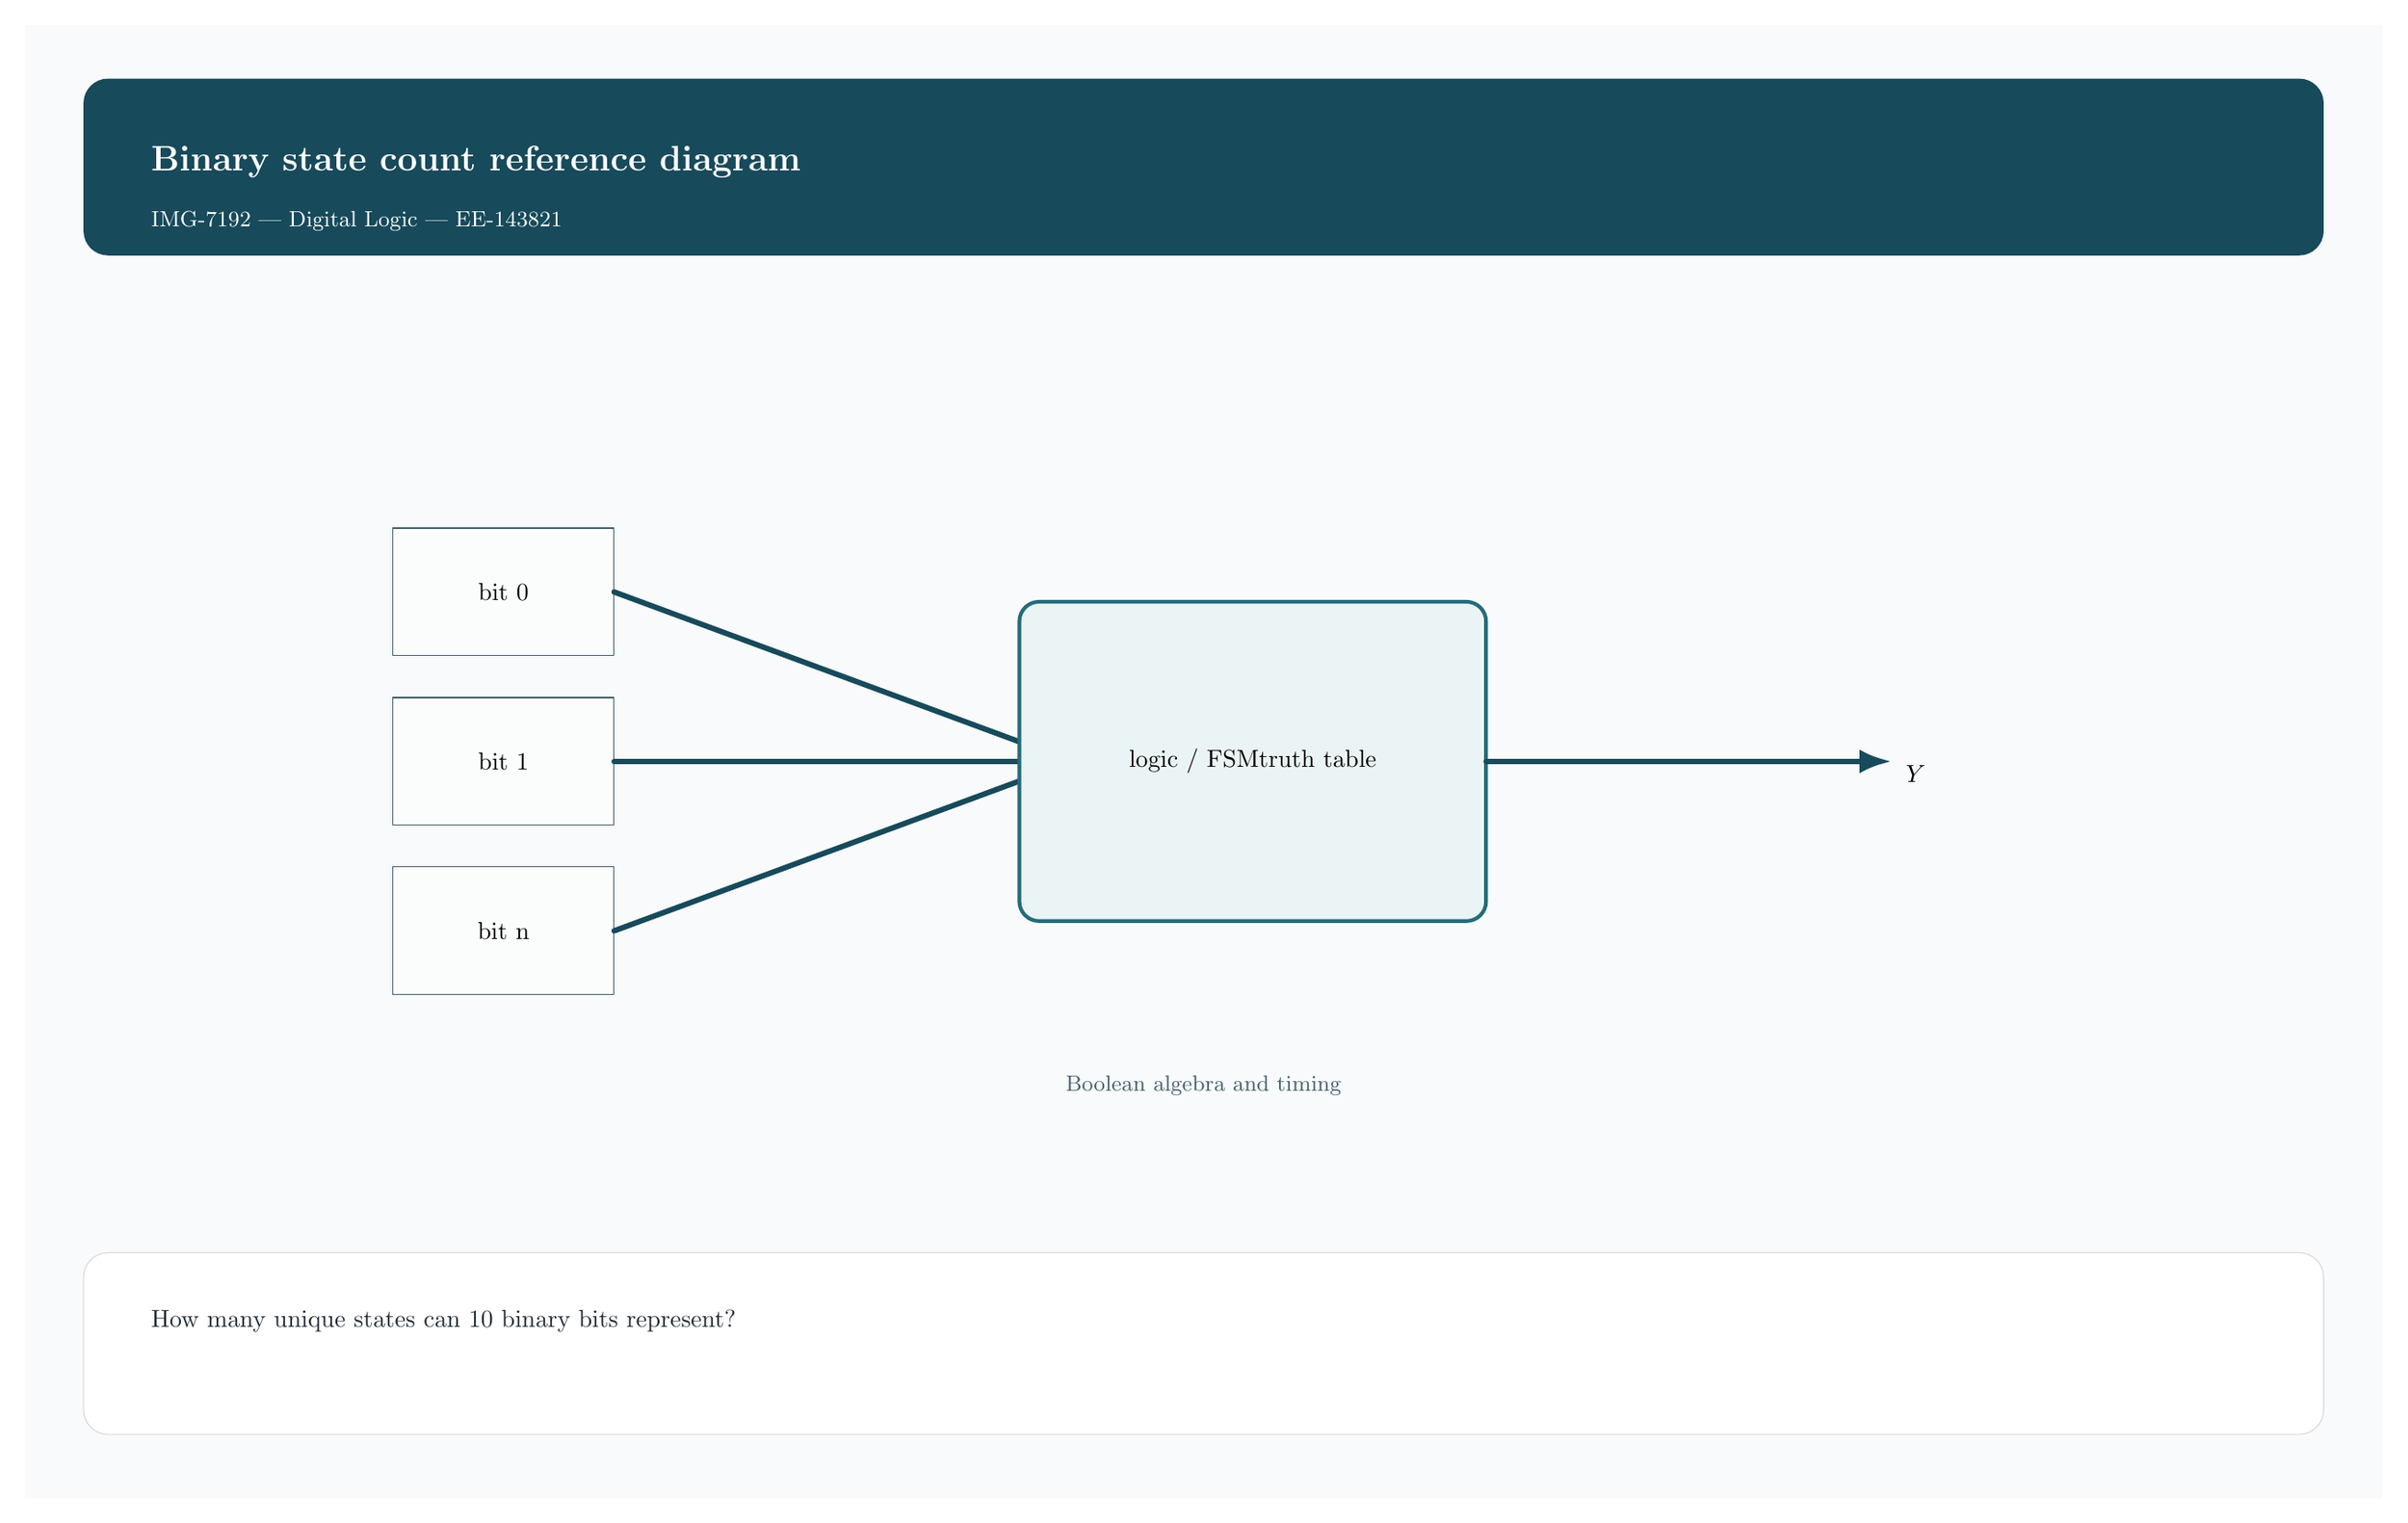
\begin{tikzpicture}[x=1pt,y=-1pt,>=Latex,line cap=round,line join=round]
\path[fill=zyloPaper] (0,0) rectangle (960,600);
\path[fill=zyloTeal,rounded corners=10pt] (24,22) rectangle (936,94);
\node[anchor=west,text=white,font=\bfseries\Large] at (48,56) {Binary state count reference diagram};
\node[anchor=west,text=white!82,font=\small] at (48,80) {IMG-7192 | Digital Logic | EE-143821};
\tikzset{wire/.style={draw=zyloTeal,line width=2.2pt},thinwire/.style={draw=zyloLine,line width=1.35pt},accent/.style={draw=zyloOrange,line width=2.2pt},box/.style={draw=zyloTealTwo,fill=zyloSoft,line width=1.5pt,rounded corners=8pt}}
\node[draw=zyloLine,fill=white!80!zyloSoft,minimum width=90pt,minimum height=52pt] at (195,231) {bit 0};
\node[draw=zyloLine,fill=white!80!zyloSoft,minimum width=90pt,minimum height=52pt] at (195,300) {bit 1};
\node[draw=zyloLine,fill=white!80!zyloSoft,minimum width=90pt,minimum height=52pt] at (195,369) {bit n};
\draw[wire] (240,231) -- (405,292); \draw[wire] (240,300) -- (405,300); \draw[wire] (240,369) -- (405,308);
\node[box,minimum width=190pt,minimum height=130pt] at (500,300) {logic / FSM\\truth table};
\draw[wire,->] (595,300) -- (760,300); \node at (770,305) {$Y$};
\node[font=\small,text=zyloLine] at (480,432) {Boolean algebra and timing};
\path[draw=black!15,fill=white,rounded corners=10pt] (24,500) rectangle (936,574);
\node[anchor=west,text width=860pt,align=left,text=zyloInk,font=\normalsize] at (48,528) {How many unique states can 10 binary bits represent?};
\end{tikzpicture}
\end{document}
